This chapter summarises and reflects upon the project as a whole, discussing the various aspects that went well and those that can be improved. The initial project aims defined in the Introduction in Section \ref{sec:introduction-project-aims} are first reviewed, followed by the future work for the project. Finally, the chapter concludes with an analysis of the limitations of the current project and a future commercial application before ending with general reflections about what was accomplished and learned through this project.

%%%%%%%%%%%%%%%%%%%%%%%%%%%%%%%%%%%%%%%%%%%%%%%%%%%%%%%%%%%%%%%%%%%%
%%%%%%%%%%%%%%%%%%%%%%%%%%%%%%%%%%%%%%%%%%%%%%%%%%%%%%%%%%%%%%%%%%%%
%%%%%%%%%%%%%%%%%%%%%%%%%%%%%%%%%%%%%%%%%%%%%%%%%%%%%%%%%%%%%%%%%%%%

\section{Achievements}

The main goal of this project was to design and implement a prototype system to tackle the problem of exponential unstructured data growth in the form of a content-based video retrieval system oriented towards matching mobile-recorded video queries to a movie. After investigating a wide array of potential feature extraction and comparison methods to combine in order to come up with a unique solution, a functional system divided into three phases was created. The first phase processed the videos in the databases to generate compact signatures by extracting colour features and storing them in histograms. The second phase repeated the process with an input query video that is matched to one of the database videos by calculating the distances between the videos' compact signatures. Finally, the third phase was dedicated to making the system suitable for movies by segmenting the videos in the database through a shot boundary detection algorithm.\\

This pipeline of three phases that constituted the system produced positive results with a custom database of 50 videos ranging from 7 to 14 seconds. Indeed, it accurately found the correct matches to queries recorded with a mobile device that included undesired camera movement and poor framing (recorded at a distance and an angle from the screen) with accuracies reaching a maximum of 93.18\%. However, the system fell short when dealing with unfavourable environmental conditions such as the non-white light sources in dark environments and light reflections glaring on the screen, with a minimum of 45.45\% accuracy and in some extreme cases, mismatches.\\

Unfortunately, the system could not be tested with a database of movies due to availability and licensing constraints, but a single movie was used to test the database pre-processing phase of the system. The movie was reduced to less than 1\% of its original size thanks to the shot boundary detection algorithm, which could be used as one of the database videos in the two other phases, thus showing the links between the pipeline phases. Overall, almost every aim initially set in Section \ref{sec:introduction-project-aims} was achieved, with the exception of testing the system with a database of movies and creating an actual link between the database pre-processing and the offline feature extraction phases which was only conceptualised.
    
%%%%%%%%%%%%%%%%%%%%%%%%%%%%%%%%%%%%%%%%%%%%%%%%%%%%%%%%%%%%%%%%%%%%
%%%%%%%%%%%%%%%%%%%%%%%%%%%%%%%%%%%%%%%%%%%%%%%%%%%%%%%%%%%%%%%%%%%%
%%%%%%%%%%%%%%%%%%%%%%%%%%%%%%%%%%%%%%%%%%%%%%%%%%%%%%%%%%%%%%%%%%%%

\section{Future Work}

A lot of different aspects that were skipped due to time constraints can be added to the system in its current state to improve the runtime and accuracy in order to ultimately use larger databases and longer videos.

\subsection{Current Pipeline Improvements}

Many improvements could be accomplished while keeping the original system's design concepts laid out in Chapter \ref{ch:chapter4}, including the colour-based features and distance metric calculations. The first change involves the histograms. Rather than generating averaged global histograms for each shot, region-based histograms should be generated instead. For example, the frames used to generate the histograms can be divided into several regions, and an average histogram could be generated for each region. This would ensure a much higher level of accuracy when matching the query video to a database video as the histograms no longer describe the colour distribution throughout the entire image but for a smaller localised region. For example, if the two frames contain both 40\% of blue, where one corresponds to the sky and one to the sea, then a global histogram would not be able to differentiate the two frames easily, whereas a region-based histogram would as the blues would not be in the same region. An illustration of a frame segmented into five distinct regions can be found in Figure \ref{fig:conclusions-image_regions}.\\

\begin{figure}[h] 
\centerline{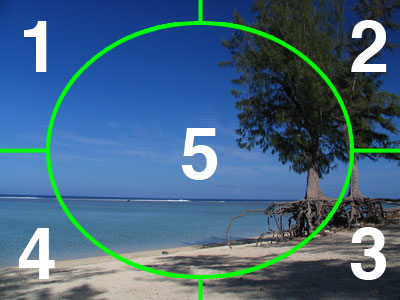
\includegraphics[width=0.5\textwidth]{figures/conclusions/image_regions.jpg}}
\caption{\label{fig:conclusions-image_regions}Example of a frame segmented into 5 regions.}
\end{figure}

Additionally, histogram models that do not produce accurate results, such as the greyscale and RGB histograms, could be excluded from future versions. Instead, only HSV histograms and new histograms with similar levels of complexity such as HSL\footnote{Hue Saturation Lightness} histograms could be used to maintain high accuracy. Indeed, considering the queries used in Chapter \ref{ch:chapter6}, if only the HSV histograms with the EMD and energy distance metrics were used, 100\% would be achieved for every single query. One of the observations from Section \ref{sec:evaluation-histogram-models-and-distance-metrics-analysis} is that the minimum accuracy of 45.45\% achieved is due to the HSV histograms outweighing the greyscale and RGB histograms thanks to the pre-assigned weights from Table \ref{tab:distance-metric-weights}. Therefore, using only similar histogram models and distance metrics would increase the performance of the system both in terms of accuracy and runtime since fewer histograms would need to be generated and fewer distances to be calculated.

\subsection{Interface-Related Improvements}

In terms of interface, simple changes can be carried out to make the system more usable, without the need to create a marketable mobile application yet. The first change is the interface itself, replacing the CLI with a GUI. A GUI would allow the results to be displayed more easily on the screen along with more straightforward interactions through button presses rather than console argument parsing. The generated data, such as the matched video, the histograms and the results tables would be more easily accessible and readable. Improving the system to a GUI could be done using either Tkinter, the native GUI library for Python if it remains the programming language used, or by rendering a clean HTML webpage.\\

Regarding the manual ROI selection, two improvements could be made. The first is a simple enhancement to allow four distinct points to be chosen to select the region of interest. Currently, allowing only two points limits the ROI to be a rectangle which cannot be rotated. Supporting four points would allow quadrilateral shapes other than rectangles to be picked and rotated. This would significantly boost the performance of the online retrieval phase since skewed queries could be cropped without losing any information and queries with undesired artefacts such as light reflections on the edges of the screen could be easily pruned.\\

An improvement that was not implemented as it was outside the project scope is automatic ROI selection. Eventually, in a commercial application, edges could be detected using horizontal and vertical Sobel operators to outline the contour of the screen, and once the edges are determined pixels outside the area could be excluded. This could not be implemented due to the sheer complexity of integrating such a feature, which could be a dissertation project on its own.

\subsection{System Redesign for Large-Scale Databases}

Moving away from the current system pipeline developed as part of this project, fundamental changes need to be applied. The simple choice of features and model used to build the system functions well with small databases of short videos, but in order to build a system that could work with larger databases and movies, significant modifications to these need to be made. The first change concerns the types of features. Indeed, more advanced features such as shape-based, motion and object features need to be extracted rather than extracting only colours. The second change consists in implementing more advanced learning models, such as Bags-of-Visual-Words or neural networks to more efficiently train and test the system with more data. 

%%%%%%%%%%%%%%%%%%%%%%%%%%%%%%%%%%%%%%%%%%%%%%%%%%%%%%%%%%%%%%%%%%%%
%%%%%%%%%%%%%%%%%%%%%%%%%%%%%%%%%%%%%%%%%%%%%%%%%%%%%%%%%%%%%%%%%%%%
%%%%%%%%%%%%%%%%%%%%%%%%%%%%%%%%%%%%%%%%%%%%%%%%%%%%%%%%%%%%%%%%%%%%

\section{Limitations}
\label{sec:conclusions-limitations}

\subsection{Project Limitation}

The main limitation of this dissertation project is the time constraint. Due to the short amount of time available to design and implement a functional system, many compromises had to be made to develop a prototype that could be tested. For this reason, plenty of various aspects had to be either be simplified or skipped. The first main compromise came within the features to extract from the video. As mentioned in the literature review, a lot of potential features could be extracted to represent a video, ranging from static to dynamic features. Colour-based features were chosen, but complementing the system with dynamic features as well would have significantly increased its accuracy. However, these being much more complex to extract and compare efficiently, thus could not be included in the code. A second compromise made was regarding the learning model. The simplest option available, corresponding to storing the extracted features into histograms which were then compared using distance metrics to find the closest one to the query, was elected to accommodate a small database. More complete models such as Bags-of-Visual-Words and deep learning models (e.g. neural networks) could not be considered due to their complexity and the time required to implement them. Indeed, the focus was to create a functional system by developing the different phases of a pipeline without necessarily coding all the intermediate steps. For instance, third-party libraries were used for the essential computer vision functions and the video stabilisation, while other aspects were simplified such as an intuitive interface replaced by a simple command line interface or automatic ROI selection replaced by manual cropping.

\subsection{Commercial Application Limitations}

The leading limitation of a future marketable application to match movies lies within the nature of the data itself. Indeed, videos, and in particular movies, are substantial objects. No matter the efficiency of the algorithm, processing them requires a lot of time and computing power, which is not always available. This fact is verified with the evaluation test carried out in Section \ref{sec:evaluation-movie-segmentation-test}, where pre-processing a single feature-length movie took an average of 2 hours and 35 minutes. This step includes the actual visual content extraction to represent a movie with features. Given a database of at least 100,000 movies, which would be a realistic number to start a commercial movie matching application, the amount of time to pre-process and later train the model would be colossal and unrealistic. Additionally, publicly available databases of movies do not exist due to copyright and legal issues, as most of them are owned by studios that only sell viewing rights to streaming services. Therefore, coming up with a database of movies with enough relevant titles to make the application interesting would be a challenge on its own.
    
%%%%%%%%%%%%%%%%%%%%%%%%%%%%%%%%%%%%%%%%%%%%%%%%%%%%%%%%%%%%%%%%%%%%
%%%%%%%%%%%%%%%%%%%%%%%%%%%%%%%%%%%%%%%%%%%%%%%%%%%%%%%%%%%%%%%%%%%%
%%%%%%%%%%%%%%%%%%%%%%%%%%%%%%%%%%%%%%%%%%%%%%%%%%%%%%%%%%%%%%%%%%%%

\section{Project Summary \& Reflections}

This project focused on multiple interests of mine by combining movies with programming. The main inspiration for this project originated from the goal to re-create the music matching application \textit{``Shazam''} for movies. With the main limitations mentioned in Section \ref{sec:conclusions-limitations} already known before starting the project, it was an exciting challenge to explore how the system could be designed and to create a functional prototype that could be tested and showcased to teachers, friends and family.\\

The code developed for this dissertation can be found online at the following URL: \url{https://github.com/Adamouization/Content-Based-Video-Retrieval-Code}.